\documentclass{beamer}
% \usepackage[TU]{fontenc}
\usepackage{lmodern} % load a font with all the characters
% \usepackage{unicode-math}

\setlength{\parskip}{\baselineskip} 

% Essential packages
\usepackage[english,danish]{babel}
\usepackage[utf8]{inputenc}
\usepackage{textcomp}
\usepackage[skins,minted,breakable]{tcolorbox}
\usepackage{booktabs}
\usepackage{pifont}

% Math packages
\usepackage{amsmath,amsfonts,amssymb,amsthm}
\usepackage{pgfplots}
\usepackage{pgfplotstable}

% Programming packages
\usepackage{listings,newtxtt}
\usepackage[ruled,vlined,linesnumbered]{algorithm2e}
\usepackage{courier}

% Layout packages
\usepackage{csquotes}
\usepackage{booktabs}
\usepackage{multicol}
\usepackage{graphicx}
\usepackage{fancyhdr}
\usepackage{lipsum}
\usepackage{subcaption}
\usepackage[style=numeric-comp,maxbibnames=99]{biblatex}
\usepackage{forest}
\usepackage{array}
\usepackage{colortbl}
\usepackage{outlines}

\usepackage{tikz}  
\usetikzlibrary{
    calc,
    matrix,
    chains,
    positioning,
    arrows.meta,
    bending,
    shapes.arrows,
    calc,
    positioning,
    backgrounds,
    decorations.pathreplacing,
    calligraphy,
}

\addbibresource{bibliography.bib}
\addbibresource{iacr.bib}

\newcommand{\eff}{\mathbb{F}} % Fancy F
\newcommand{\pp}{\texttt{++}} % ++ operator
\newcommand{\rightshift}{\texttt{ >> }} 
\newcommand{\td}[1]{\todo[inline]{#1}} % Todo notes
\newcommand{\cmark}{\ding{51}}%
\newcommand{\xmark}{\ding{55}}%

\title{Implementation and Evaluation of Dinur's MQ Solver Algorithm}
\author{Author: Mikkel Juul Vestergaard\\Supervisor: Associate Professor Ruben Niederhagen}
\institute{Department of Mathematics and Computer Science\\University of Southern Denmark}
\date{Thesis Defence, 2023}

\AtBeginSubsection[]
{
  \begin{frame}
    \frametitle{Table of Contents}
    \tableofcontents[sectionstyle=show/shaded,subsectionstyle=show/shaded/hide]
  \end{frame}
}

\begin{document}

\frame{\titlepage}

\section{Preface}
\begin{frame}
    \frametitle{The goals of this thesis.}
    Goals:
    \begin{itemize}
        \item Environment for solving systems of multivariate polynomials using Itai Dinur's.polynomial-method algorithm.
        \item Software should run on desktop computers, HPC hosts, or a subset of these.
        \item Host-specific traits for implementation.
        \item Extendable code.
        \item Performance capture.
        \item Report shedding light on the practical performance of the algorithm.
    \end{itemize}
\end{frame}

\section{Introduction}
\subsection{Polynomials 101}
\begin{frame}
    \frametitle{Polynomials?}
    A mathematical expression or function in some variable(s), coefficients and declared through the operators:
    \begin{itemize}
        \item Addition.
        \item Subtraction.
        \item Multiplication.
        \item Exponentiation using non-negative integers.
    \end{itemize}
\end{frame}

\begin{frame}
    \frametitle{Polynomials.}
    Some simple polynomials as mathematical functions:
    \begin{equation*}
        \begin{split}
            p(x) &= 4x + 1\\
            f(x) &= 2x^2 + 3
        \end{split}
    \end{equation*}
    and expressions:
    \begin{equation*}
        \begin{split}
            &x^{10}\\
            &x^5 + 10x^3
        \end{split}
    \end{equation*}

\end{frame}

\begin{frame}
    \frametitle{Multivariate polynomials.}
    So, what are these \textit{multivariate} polynomials?
    
    \pause 

    Well, just polynomials in \textit{multiple} variables!

    \pause 

    Typically we denote these variables by subscript (of course starting from $0$).

    E.g. $x_0, x_1, \dots x_{n - 1}$, however, we can still of course call them $x, y, z$, etc.

    \pause 

    For a notational shorthand, 
    $$
        \mathbf{x} = (x_0, x_1, \dots x_{n - 1})
    $$ 
    for $n$ variables, and likewise for variables denoted by $y$s and $z$s.
\end{frame}

\begin{frame}
    \frametitle{Multivariate polynomials.}
    So how do these look?

    \pause 

    Quite simply, they look like the polynomials we just saw but with more variables!

    \pause 
    For example:
    \begin{equation*}
        \begin{split}
            p_0(x_0, x_1, x_2, x_3) &= 5x_3^4 + x_0^2 + 4x_1 + 10\\
            p_1(x_0, x_1, x_2, x_3) &= 3x_1x_2x_3 + 2x_0^2
        \end{split}
    \end{equation*}
\end{frame}

\begin{frame}
    \frametitle{Boolean multivariate polynomials!}
    But in fact, sometimes we want to restrict multivariate polynomials. How may we do that?

    \pause 

    We may restrict the \textit{coefficients} and \textit{variable} assignments.
    
    In this case, the coefficients are restricted to $0$s and $1$s, and the same goes for the assignments we can make to the variables!

    \pause 

    I.e. we restrict the multivariate polynomials to look like 
    \begin{equation*}
        \begin{split}
            &x_0x_1 + x_0\\
            &x_0^2 + x_1x_2
        \end{split}
    \end{equation*}
    \pause 
    
    Polynomials of this sort are often called \textit{boolean} polynomials, or in this case \textit{boolean multivariate polynomials}.
\end{frame}

\begin{frame}
    \frametitle{Boolean multivariate polynomials! (Extended)}
    The operations of multiplication and addition in this context are a bit different.

    \pause 

    Mathematically, we say that these operations are performed \textit{modulo two}. However, this simply means that we \textit{wrap} any operations with a result larger than one around to zero. E.g. $1 + 1 + 1 = 1$ (as $1 + 1 = 0$).

    Multiplication is as we know, with $1 \cdot 1 = 1$ and $0 \cdot 1 = 0$.
\end{frame}

\subsection{What is the ''MQ-problem''?}
\begin{frame}
    \frametitle{The MQ-problem}
    Well, the MQ-problem relates to multivariate polynomials. How so, you ask?
    \pause
    \begin{outline}
        \1 A system of boolean multivariate polynomials.
            \2 $m$ polynomials. 
            \2 $n$ variables.
            \2 The polynomials are of degree $d$.
            \2 Coefficients are $0$ or $1$.
            \2 From this point on, systems of polynomials are written as $\mathcal{P} = \{p_0, p_1, p_2, \dots p_{m-1}\}$
    \end{outline}

    \pause 

    We typically say that a \textit{solution} to a system $\mathcal{P}$ is an assignment of the variables of the polynomial s.t. 
    $$
        p_{0}(\hat{\mathbf{x}}) = p_{1}(\hat{\mathbf{x}}) = \dots = p_{n-1}(\hat{\mathbf{x}}) = 0
    $$
\end{frame}

\begin{frame}
    \frametitle{The MQ-problem}
    All right, why bother?
    \pause
    \begin{outline}
        \1 Solving systems of multivariate polynomials (in general) is hard for a computer!
            \2 We often denote $MP$ as the problem of solving multivariate polynomials of degree $d$ in $n$ variables and $m$ polynomials.

        \pause 

        \1 A commonly used version of the $MP$-problem is the $MQ$-problem.
            \2 This is the problem of solving systems of $m$ quadratic polynomials in $n$ variables.
            \2 This is also very hard for a computer to solve while having nice properties for real implementations.
            \2 Much modern cryptography is based on the hardness of this problem.
    \end{outline}
\end{frame}

\subsection{The algorithm}
\begin{frame}
    \frametitle{Dinur's algorithm}
    In \cite{eurocrypt-2021-30841}, Dinur proposed an algorithm for $MP$ problems with \textbf{exponential speedup} over exhaustive search.

    The algorithm is based on the \textit{polynomial-method}, which is borrowed from circuit complexity.

    To the best of my knowledge, this algorithm has not been tested in practice.

    It borrows ideas from other algorithms based on the same method.
\end{frame}

\begin{frame}
    \frametitle{The Polynomial method}
    Algorithms based on the polynomial method solve systems 
    $$
        \mathcal{P} = \{p_j(\mathbf{x})\}^{m - 1}_{j = 0}
    $$ 
    by considering constructing a polynomial 
    $$
        F(\mathbf{x}) = (1 + p_0(\mathbf{x}))(1 + p_1(\mathbf{x})) \dots (1 + p_{m - 1}(\mathbf{x}))
    $$
    with multiplication and addition acting as noted earlier.

    Notice how a solution to $\mathcal{P}$ evaluates to $1$ on $F$.
\end{frame}

\begin{frame}
    \frametitle{The Polynomial method}
    However, since $F$ may have a rather high degree ($m \cdot d$), the methods may instead \textit{generate} a related system, 
    $$
        \Tilde{\mathcal{P}}_k \gets \left\{r_i(\mathbf{x}) = \sum_{j = 0}^{m-1}A_{i,j} \cdot p_j(\mathbf{x})\right\}^{\ell - 1}_{i = 0},
    $$
    with a random matrix $A$ of rank $\ell$, which allows for constructing the \textit{probabilistic polynomial}
    $$
        \Tilde{F}(\mathbf{x}) = (1 + r_0(\mathbf{x}))(1 + r_1(\mathbf{x})) \dots (1 + r_{\ell - 1}(\mathbf{x})) 
    $$
    of smaller degree ($d \cdot \ell$), assuming one chooses an $\ell < m$.
\end{frame}

\begin{frame}
    \frametitle{Isolating solutions}
    \begin{block}{Variable partition}
        For the variables $\mathbf{x} = (x_0, \dots x_{n - 1})$, we make the partition $\mathbf{x} = (\mathbf{y}, \mathbf{z}) = (y_0, \dots y_{n - n_1 - 1}, z_{0}, \dots z_{n_1 - 1})$ using some parameter $n_1$.
    \end{block}

    \begin{alertblock}{Isolated solutions}
        A solution $\hat{\mathbf{x}} = (\hat{\mathbf{y}},\hat{\mathbf{z}})$ to a system $\mathcal{P} = \{p_j(\mathbf{y}, \mathbf{z})\}^m_{j = 1}$ is called \textit{isolated} (with respect to the variable partitition $(\mathbf{y}, \mathbf{z})$) if for all $\hat{\mathbf{z}}'=\hat{\mathbf{z}}$, $(\hat{\mathbf{y}}, \hat{\mathbf{z}}')$ is not a solution to $\mathcal{P}$.
    \end{alertblock}
    What if we, instead of searching for \textit{any} solution, search for an isolated solution? 
\end{frame}

\begin{frame}
    \frametitle{Isolating solutions, why?}
    Let us consider a system with polynomials $p_0$ and $p_1$, over $6$ variables. 

    \pause
    Say we split the variables so that the first four variables are the $\mathbf{y}$-variables, and the last two variables are the $\mathbf{z}$-variables. I.e. 
    $$
        ({\color{cyan}x_0}, {\color{cyan}x_1}, {\color{cyan}x_2}, {\color{cyan}x_3}, {\color{purple}x_4}, {\color{purple}x_5}) = ({\color{cyan}y_0}, {\color{cyan}y_1}, {\color{cyan}y_2}, {\color{cyan}y_3}, {\color{purple}z_0}, {\color{purple}z_1})
    $$
    with colors denoting $\color{cyan}\mathbf{y}$-variables and $\color{purple}\mathbf{z}$-variables.
\end{frame}

\begin{frame}
    \frametitle{Isolating solutions, why?}
    Now, let us examine the following examples
    \begin{equation*}
        \begin{split}
            &p_0({\color{cyan}1}, {\color{cyan}1}, {\color{cyan}1}, {\color{cyan}0}, {\color{purple}0}, {\color{purple}0}) = 0, p_1({\color{cyan}1}, {\color{cyan}1}, {\color{cyan}1}, {\color{cyan}0}, {\color{purple}0}, {\color{purple}0}) = 0 \uncover<2->{\text{ \color{green}\cmark}}\\
            &p_0({\color{cyan}1}, {\color{cyan}1}, {\color{cyan}1}, {\color{cyan}0}, {\color{purple}0}, {\color{purple}1}) = 1, p_1({\color{cyan}1}, {\color{cyan}1}, {\color{cyan}1}, {\color{cyan}0}, {\color{purple}0}, {\color{purple}1}) = 0 \uncover<3->{\text{ \color{red}\xmark}}\\
            &p_0({\color{cyan}1}, {\color{cyan}1}, {\color{cyan}1}, {\color{cyan}0}, {\color{purple}1}, {\color{purple}0}) = 0, p_1({\color{cyan}1}, {\color{cyan}1}, {\color{cyan}1}, {\color{cyan}0}, {\color{purple}1}, {\color{purple}0}) = 1 \uncover<4->{\text{ \color{red}\xmark}}\\
            &p_0({\color{cyan}1}, {\color{cyan}1}, {\color{cyan}1}, {\color{cyan}0}, {\color{purple}1}, {\color{purple}1}) = 1, p_1({\color{cyan}1}, {\color{cyan}1}, {\color{cyan}1}, {\color{cyan}0}, {\color{purple}1}, {\color{purple}1}) = 0 \uncover<5->{\text{ \color{red}\xmark}}
        \end{split}
    \end{equation*}
    and 
    \begin{equation*}
        \begin{split}
            &p_0({\color{cyan}1}, {\color{cyan}0}, {\color{cyan}0}, {\color{cyan}1}, {\color{purple}0}, {\color{purple}0}) = 0, p_1({\color{cyan}1}, {\color{cyan}0}, {\color{cyan}0}, {\color{cyan}1}, {\color{purple}0}, {\color{purple}0}) = 0 \uncover<6->{\text{ \color{green}\cmark}}\\
            &p_0({\color{cyan}1}, {\color{cyan}0}, {\color{cyan}0}, {\color{cyan}1}, {\color{purple}0}, {\color{purple}1}) = 0, p_1({\color{cyan}1}, {\color{cyan}0}, {\color{cyan}0}, {\color{cyan}1}, {\color{purple}0}, {\color{purple}1}) = 1 \uncover<7->{\text{ \color{red}\xmark}}\\
            &p_0({\color{cyan}1}, {\color{cyan}0}, {\color{cyan}0}, {\color{cyan}1}, {\color{purple}1}, {\color{purple}0}) = 0, p_1({\color{cyan}1}, {\color{cyan}0}, {\color{cyan}0}, {\color{cyan}1}, {\color{purple}1}, {\color{purple}0}) = 0 \uncover<8->{\text{ \color{green}\cmark}}\\
            &p_0({\color{cyan}1}, {\color{cyan}0}, {\color{cyan}0}, {\color{cyan}1}, {\color{purple}1}, {\color{purple}1}) = 1, p_1({\color{cyan}1}, {\color{cyan}0}, {\color{cyan}0}, {\color{cyan}1}, {\color{purple}1}, {\color{purple}1}) = 0 \uncover<9->{\text{ \color{red}\xmark}}
        \end{split}
    \end{equation*}
\end{frame}

\begin{frame}
    \frametitle{Recovering bits}
        By partitioning the variables using the parameter $n_1$, we are able to \textit{enumerate} all isolated solutions of the partition using the polynomials
        $$
            U_0(\mathbf{y}) = \sum_{\hat{\mathbf{z}} \in \{0,1\}^{n_1}} \Tilde{F}(\mathbf{y},\hat{\mathbf{z}}), \text{ and } U_i(\mathbf{y}) = \sum_{\hat{\mathbf{z}}\in \{0,1\}^{n_1 - 1}} \Tilde{F}_{z_i \leftarrow 0}(\mathbf{y}, \hat{\mathbf{z}}),
        $$
        for $i = 1, \dots n_1$. \pause

        Using the $U$ polynomials above, it turns out that $U_0(\hat{\mathbf{y}}) = 1$ tells us that $(\hat{\mathbf{y}}, \hat{\mathbf{z}})$ is an \textit{isolated solution}! But what is $\hat{\mathbf{z}}$?

        \pause 

        Actually, it is $U_i(\hat{\mathbf{y}}) = z_{i - 1} + 1$, i.e. $U_i$ (for $i = 1, \dots n_1$) can \textit{recover} the $\mathbf{z}$-bits of an isolated solution.
\end{frame}

\begin{frame}
    \frametitle{Example search}
    \begin{equation*}
        \begin{split}
            \only<1>{&p_0({\color{cyan}0}, {\color{cyan}0}, {\color{cyan}0}, {\color{cyan}0}, {\color{purple}?}, {\color{purple}?})\\
            &p_1({\color{cyan}0}, {\color{cyan}0}, {\color{cyan}0}, {\color{cyan}0}, {\color{purple}?}, {\color{purple}?})}
            \only<2>{&p_0({\color{cyan}1}, {\color{cyan}0}, {\color{cyan}0}, {\color{cyan}0}, {\color{purple}?}, {\color{purple}?})\\
            &p_1({\color{cyan}1}, {\color{cyan}0}, {\color{cyan}0}, {\color{cyan}0}, {\color{purple}?}, {\color{purple}?})}
            \only<3>{&p_0({\color{cyan}1}, {\color{cyan}1}, {\color{cyan}0}, {\color{cyan}0}, {\color{purple}?}, {\color{purple}?})\\
            &p_1({\color{cyan}1}, {\color{cyan}1}, {\color{cyan}0}, {\color{cyan}0}, {\color{purple}?}, {\color{purple}?})}
        \end{split}
    \end{equation*}

    \begin{equation*}
        \begin{split}
            \only<1>{
                U_0({\color{cyan}0}, {\color{cyan}0}, {\color{cyan}0}, {\color{cyan}0}) &= 0 \text{ \color{red}\xmark}\\
                U_1({\color{cyan}0}, {\color{cyan}0}, {\color{cyan}0}, {\color{cyan}0}) &= {\color{purple}z_0} + 1 = \text{?}\\
                U_2({\color{cyan}0}, {\color{cyan}0}, {\color{cyan}0}, {\color{cyan}0}) &= {\color{purple}z_1} + 1 = \text{?}
            }
            \only<2>{
                U_0({\color{cyan}1}, {\color{cyan}0}, {\color{cyan}0}, {\color{cyan}0}) &= 0 \text{ \color{red}\xmark}\\
                U_1({\color{cyan}1}, {\color{cyan}0}, {\color{cyan}0}, {\color{cyan}0}) &= {\color{purple}z_0} + 1 = \text{?}\\
                U_2({\color{cyan}1}, {\color{cyan}0}, {\color{cyan}0}, {\color{cyan}0}) &= {\color{purple}z_1} + 1 = \text{?}
            }
            \only<3>{
                U_0({\color{cyan}1}, {\color{cyan}1}, {\color{cyan}0}, {\color{cyan}0}) &= 1 \text{ \color{green}\cmark}\\
                U_1({\color{cyan}1}, {\color{cyan}1}, {\color{cyan}0}, {\color{cyan}0}) &= {\color{purple}z_0} + 1 = 0\\
                U_2({\color{cyan}1}, {\color{cyan}1}, {\color{cyan}0}, {\color{cyan}0}) &= {\color{purple}z_1} + 1 = 1
            }
        \end{split}
    \end{equation*}
    
    \onslide<3>{$({\color{cyan}y_0}, {\color{cyan}y_1}, {\color{cyan}y_2}, {\color{cyan}y_3}, {\color{purple}z_0}, {\color{purple}z_1}) = ({\color{cyan}1}, {\color{cyan}1}, {\color{cyan}0}, {\color{cyan}0}, {\color{purple}1}, {\color{purple}0})$ is an isolated solution to the system $\{p_0, p_1\}$}.
    
\end{frame}

\begin{frame}
    \frametitle{Interpolation}
    The sums for the $U$ polynomials are unwieldy and hard to compute in practice! In fact, up to $2^{n_1}$ evaluations of $\Tilde{F}$ needs to be computed for \textit{each} input to the $U$ polynomials.

    \pause 

    Alternatively, we may interpolate (obtain a mathematical expression) the $U$s directly and then evaluate them.

    \pause 

    We may do this using something called the \textit{Möbius transform}.
\end{frame}

\begin{frame}[fragile]
    \frametitle{Möbius transforms}
    The Möbius transform can take as input the evaluations of a polynomial and can be used to output a mathematical expression of it.
    \pause
\begin{figure}[t]
    \centering 
    \begin{tikzpicture}[
        % every node/.style={minimum height=2em}
    ]
        \matrix [
            matrix of math nodes,
            nodes={
                sharp corners,
                outer sep=0pt,
                anchor=center,
            },
        ] (mat) {
            x_0 & x_1   & p(x_0, x_1)\\ 
            \hline\\
            0   & 0     & 0\\ 
            \hline\\
            1   & 0     & 0\\
            \hline\\
            0   & 1     & 1\\
            \hline\\
            1   & 1     & 1\\
            \hline\\
        };

        \node[right=1.5cm of mat] (poly) {$p(x_0,x_1) = x_0 + x_1 + x_0x_1$};
        
        \only<2>{\draw [-stealth] (mat.east) -- (poly.west) node[above=10pt, pos=0.5] {};}
        \only<3>{\draw [stealth-stealth] (mat.east) -- (poly.west) node[above=10pt, pos=0.5] {};}
        
    \end{tikzpicture}
\end{figure}
\end{frame}

\section{Contributions}
\subsection{Software suite}

\begin{frame}
    \frametitle{Repository contents}
    Divided into three implementations, each with its own Makefile target.
    \begin{itemize}
        \item SageMath for algorithmic tests.
        \item Standard C implementation for more portable, but still optimized implementation.
        \item C implementation using AVX for a more ``hyper``-optimized approach.
    \end{itemize}

    The codebases can be extended by using the current header-file setup as a template.
\end{frame}

\begin{frame}
    \frametitle{Repository structure}
    \begin{forest}
        for tree={
          font=\ttfamily,
          grow'=0,
          child anchor=west,
          parent anchor=south,
          anchor=west,
          calign=first,
          edge path={
            \noexpand\path [draw, \forestoption{edge}]
            (!u.south west) +(7.5pt,0) |- node[fill,inner sep=1.25pt] {} (.child anchor)\forestoption{edge label};
          },
          before typesetting nodes={
            if n=1
              {insert before={[,phantom]}}
              {}
          },
          fit=band,
          before computing xy={l=15pt},
        }
      [MQ-Solver
        [report/]
        [inc/]
        [src/
          [c/
            [standard/]
            [vectorized/]
          ]
          [sage/]
        ]
        [test/]
      ]
      \end{forest}
\end{frame}

\subsection{FES-based interpolation}
\begin{frame}
    \frametitle{Interpolating the $U$ polynomials}
    Do we need to run the Möbius transform algorithm twice?

    \pause 

    No, we can use a FES-based interpolation instead! 
    $\implies$ We may intertwine interpolation and evaluation into a single procedure.

    \pause 

    This thesis introduced the idea of interpolating boolean polynomials using the principles and ideas of FES!

    \pause 

    Let us shortly recap those.

\end{frame}

\begin{frame}
    \frametitle{Gray codes}
    Gray code or Reflected Binary Code, is an ordering of the binary numeral system in which every subsequent value only differs in \textit{one} bit.

    \begin{center}
        \begin{tabular}{||c|c|c||}
            \hline
            Index & Binary & Gray \\
            \hline
            0 & $000_2$ & $000_2$\\
            1 & $001_2$ & $001_2$\\
            2 & $010_2$ & $011_2$\\
            3 & $011_2$ & $010_2$\\
            4 & $100_2$ & $110_2$\\
            5 & $101_2$ & $111_2$\\
            6 & $110_2$ & $101_2$\\
            7 & $111_2$ & $100_2$\\
            \hline
        \end{tabular}
    \end{center}
\end{frame}

\begin{frame}
    \frametitle{Fast exhaustive search (FES) for polynomials in $\mathbb{F}_2$}
    Say we have some polynomial $p$ in the ring $\mathbb{F}_2[x_0,\dots x_{n-1}$].
    
    \pause

    We want to find all assignments of $x_0, \dots x_{n - 1}$ that evalute to 0 on $p$ $\implies$ we want to do an exhaustive search!

    But we need to do $2^n$ iterations, each \textit{fully} evaluating a polynomial. Can we do this concretely faster?
\end{frame}

\begin{frame}
    \frametitle{Derivatives in finite fields}
    Instead of \textit{fully} evaluating the polynomial $p$ at each input, why don't we use derivatives and Gray codes? 
    
    \pause 

    Let us evaluate in Gray code order (for $n = 3$):
    \begin{equation*}
        \begin{split}
            p(0,&0,0)\\
            p(1,&0,0)\\
            p(1,&1,0)\\
            p(0,&1,0)\\
            &\vdots\\
            p(0,&0,1)
        \end{split}
    \end{equation*}
\end{frame}

\begin{frame}
    \frametitle{Derivatives in finite fields}
    Now, between each of these evaluations, only \textit{one} variable changes its value, e.g. $001_2 \rightarrow 011_2$ means that only $x_1$ changes value

    \pause

    Now, to compute some $p(\hat{\mathbf{x}})$ when only variable $x_i \in \mathbf{x}$ changes value, simply add 
    $$
        \frac{\partial p}{\partial x_i}(\hat{\mathbf{x}}),
    $$
    to the previous evaluation of $p$. 

    \pause
    
    Further, we can treat the partial derivative above as a polynomial itself, applying this idea recursively.
\end{frame}

\begin{frame}
    \frametitle{Derivatives in finite fields}
    Generally, we may compute the $j$-order partial derivative recursively, by 
    $$
        \frac{\partial^{j - 1} p}{\partial x_{\beta_0} \dots \partial x_{\beta_{j - 2}}}(\mathbf{g}_i) = Q_{x_{\beta_0} \dots x_{\beta_{j - 2}}} + \frac{\partial^j p}{\partial x_{\beta_0} \dots \partial x_{\beta_{j - 1}}}(\mathbf{g}_i).
    $$
    where $\mathbf{g}_i$ is Gray code encoding of $\mathbf{x}$ and $\beta_0, \dots \beta_{j - 1}$ encode the indices of all 1-bits in $\mathbf{x}$, limited by $j < d$.
    
    Above, $Q_{x_{\beta_0} \dots x_{\beta_{j - 2}}}$ is the \textit{stored} previous evaluation of $\frac{\partial^{j - 1} p}{\partial x_{\beta_0} \dots \partial x_{\beta_{j - 2}}}$. These values can be stored in a table, also denoted the \textit{derivative table}.
\end{frame}

\begin{frame}
    \frametitle{Derivatives in finite fields}
    Using these ideas, the authors of \cite{ches-2010-23990} managed to create an exhaustive search algorithm that is quite fast in practice.

    But what was just shown is how the procedure \textit{evaluates} polynomials, so how can it be used to \textit{interpolate} them?
\end{frame}

\begin{frame}
    \frametitle{FES-based interpolation}
    What if we \textit{backtrack} using the ideas of the fast exhaustive search algorithm?

    \pause

    That is, normally in FES, we would compute 
    $$
        \frac{\partial^{j - 1} p}{\partial x_{\beta_0} \dots \partial x_{\beta_{j - 2}}}(\mathbf{g}_i) = Q_{x_{\beta_0} \dots x_{\beta_{j - 2}}} + \frac{\partial^j p}{\partial x_{\beta_0} \dots \partial x_{\beta_{j - 1}}}(\mathbf{g}_i).
    $$
    
    \pause

    But now, we can instead compute 
    $$
        \frac{\partial^j p}{\partial x_{\beta_0} \dots \partial x_{\beta_{j - 1}}}(\mathbf{g}_i) = \frac{\partial^{j - 1} p}{\partial x_{\beta_0} \dots \partial x_{\beta_{j - 2}}}(\mathbf{g}_i) - Q_{x_{\beta_0} \dots x_{\beta_{j - 2}}}
    $$
    starting from the evaluations of $p$, and \textit{filling} the derivative table entries. 
\end{frame}

\begin{frame}
    \frametitle{FES-based interpolation}
    Using this backtracking idea we can take an evaluation of $p$ and recover the values that FES would have used to compute that evaluation.

    \pause 

    However, this will \textit{not} fully interpolate $p$ from its evaluations (truth-table), given that FES has an initialization phase.

    \pause

    But we do not actually need to fully interpolate the polynomial in this case.
\end{frame}

\begin{frame}
    \frametitle{Alternative to the Möbius transform?}
    Using this idea, we can construct a procedure that interpolates \textit{and} evaluates, mimicking the two separate calls to the Möbius transform.

    \begin{outline}
        \1 Go through all $2^{n - n_1}$ values of the $\mathbf{y}$ bits.
            \2 If the hamming weight of the $\mathbf{y}$ bits is larger than $d_{\Tilde{F}} - n_1 + 1$.
                \3 We have already interpolated the desired derivative table entries, and may now evaluate new points.
            \2 Else; if it is smaller.
                \3 Interpolate derivative table entries by \textit{backtracking} and store them. This sets the entries ready for evaluations, like traditionally in FES.
    \end{outline}
\end{frame}

\subsection{Evaluation}
\begin{frame}
    \frametitle{Memory: Standard C implementation and theoretical consumption}
    \begin{figure}[t]
        \centering
        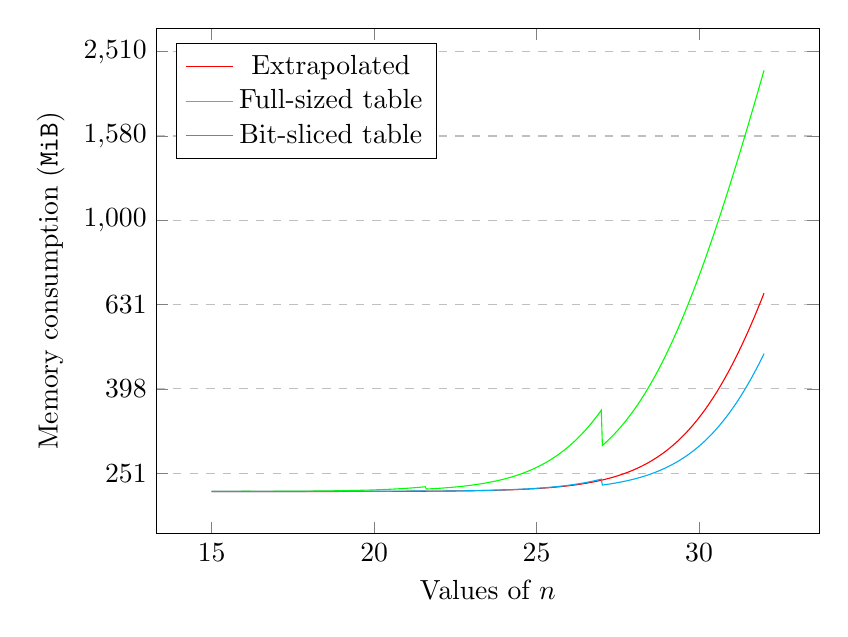
\begin{tikzpicture}
            \begin{axis}[
                xlabel=Values of $n$,
                ylabel=Memory consumption (\texttt{MiB}),
                ymode=log,
                log ticks with fixed point,
                xtick={15,20,25,30},
                height=8cm,
                width=10cm,
                ymajorgrids,
                grid style=dashed,
                legend pos=north west,
            ]
            \addplot[
                color=red,
                domain=15:32,
                samples=500,
            ]
            {(0.00013831083126693568 * 2^(0.988135062636788 * x) + 232634.0051135452)/1024};
            \addplot[
                color=green,
                domain=15:32,
                samples=500,
            ] {(4 * 8 * 2^(x - (ceil(x/5.4)))/1024 + 232634.0051135452)/1024};
            \addplot[
                color=cyan,
                domain=15:32,
                samples=500,
            ] {(4 * 2^(x - (ceil(x/5.4)))/1024 + 232634.0051135452)/1024};
            \legend{Extrapolated, Full-sized table, Bit-sliced table}
            \end{axis}
        \end{tikzpicture}
    \end{figure}
\end{frame}

\begin{frame}
    \frametitle{Memory: AVX and standard C implementations}
    \begin{figure}[t]
        \centering
        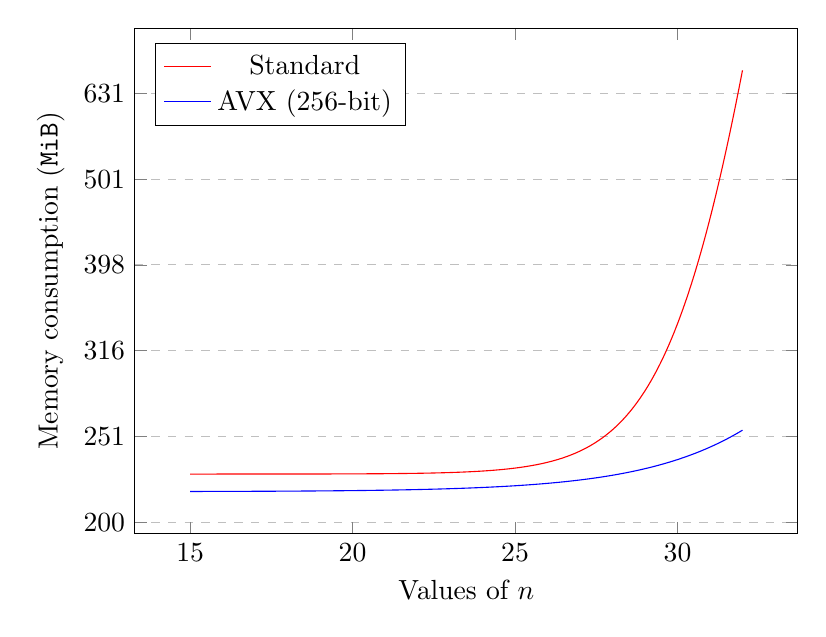
\begin{tikzpicture}
            \begin{axis}[
                xlabel=Values of $n$,
                ymode=log,
                log ticks with fixed point,
                ylabel=Memory consumption (\texttt{MiB}),
                xtick={15,20,25,30},
                height=8cm,
                width=10cm,
                ymajorgrids,
                grid style=dashed,
                legend pos=north west,
            ]
            \addplot[
                color=red,
                domain=15:32,
                samples=500,
            ]
            {(0.00013831083126693568 * 2^(0.988135062636788 * x) + 232634.0051135452)/1024};
            \addplot [
                color=blue,
                domain=15:32,
                samples=500,
            ] {(0.6300250132482776 * 2^(0.4984381599371818 * x) + 221906.00452997335)/1024};
            \legend{Standard, AVX (256-bit)}
            \end{axis}
        \end{tikzpicture}
    \end{figure}
\end{frame}

\begin{frame}
    \frametitle{Timings: Standard, AVX, and FES}
    \begin{figure}[t]
        \centering
        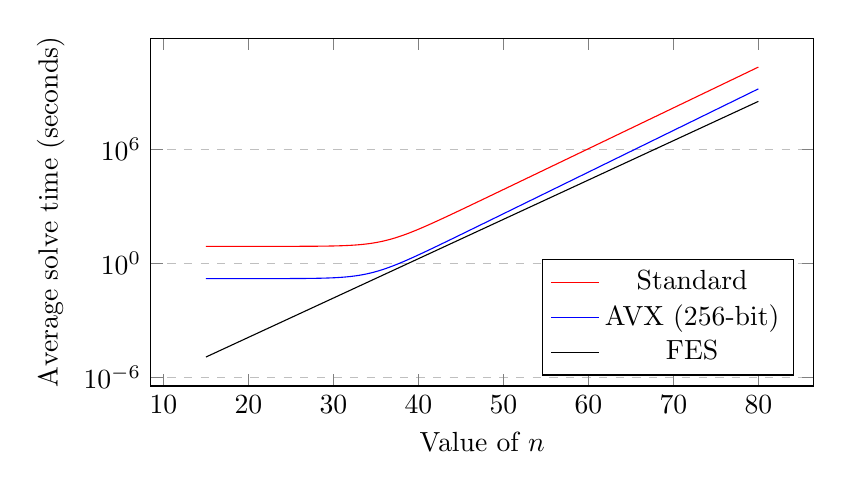
\begin{tikzpicture}
            \begin{axis}[
                xlabel={Value of $n$},
                ylabel={Average solve time (seconds)},
                ymode=log,
                ymajorgrids=true,
                grid style=dashed,
                height=6cm,
                width=10cm,
                legend pos=south east,
            ]
                \addplot [
                    color=red,
                    domain=15:80,
                    samples=500,
                ] {(0.00013821153801904347 * 2^(0.7131086234506752 * x) + 7680.492487663649)/1000};
                \addplot [
                    color=blue,
                    domain=15:80,
                    samples=500,
                ] {(4.515323644415954e-06 * 2^(0.7272699624665934 * x) + 154.55031285117195)/1000};
                \addplot [
                    color=black,
                    domain=15:80,
                    samples=500,
                ] {(9.23081156978058e-06 * 2^(0.6870633039068228 * x) + 5.026531141453392e-16)/1000};
                \legend{Standard, AVX (256-bit), FES} 
            \end{axis}
        \end{tikzpicture}
    \end{figure}
\end{frame}

\begin{frame}
    \frametitle{Timings: Standard, AVX, and FES}
    \begin{table}[t]
        \begin{center}
            \pgfplotstabletypeset[
                col sep=comma,
                columns={standard,vectorized,fes,n},
                columns/standard/.style={
                    column name=Standard,
                    postproc cell content/.append style={
                        /pgfplots/table/@cell content/.add={}{ ms}
                    },
                },
                columns/vectorized/.style={
                    column name=Vectorized,
                    postproc cell content/.append style={
                            /pgfplots/table/@cell content/.add={}{ ms}
                    },
                },
                columns/fes/.style={
                    column name=FES,
                    postproc cell content/.append style={
                        /pgfplots/table/@cell content/.add={}{ ms},
                    },
                },
                columns/n/.style={
                    column name={$n,m$},
                },   
                every even row/.style={
                    before row={
                      \rowcolor[gray]{0.9}
                    }
                },
                every head row/.style={
                    before row=\toprule,
                    after row=\midrule
                },
                every last row/.style={
                    after row=\bottomrule
                },
           ]{metrics/fes_dinur/bench_comp.csv}
        \end{center}
    \end{table}
\end{frame}

\begin{frame}
    \frametitle{Timings: FES-recovery}
    \begin{table}[t]
        \begin{center}
            \pgfplotstabletypeset[
                col sep=comma,
                columns={recovery,interpolation,evaluation,n},
                columns/recovery/.style={
                    column name=Recovery,
                    postproc cell content/.append style={
                        /pgfplots/table/@cell content/.add={}{ ms}
                    },
                },
                columns/interpolation/.style={
                    column name=Interpolation,
                    postproc cell content/.append style={
                            /pgfplots/table/@cell content/.add={}{ ms}
                    },
                },
                columns/evaluation/.style={
                    column name=Evaluation,
                    postproc cell content/.append style={
                        /pgfplots/table/@cell content/.add={}{ ms},
                    },
                },
                columns/n/.style={
                    column name={$n,m$},
                },   
                every even row/.style={
                    before row={
                      \rowcolor[gray]{0.9}
                    }
                },
                every head row/.style={
                    before row=\toprule,
                    after row=\midrule
                },
                every last row/.style={
                    after row=\bottomrule
                },
           ]{metrics/fes_dinur/bench_recover.csv}
        \end{center}
    \end{table}
\end{frame}

\begin{frame}
    \frametitle{Future works}
    Examples:
    \begin{itemize}
        \item Find the problem with amount of potential solutions.
        \item Check impact of $n_1$.
        \item Proper Möbius transform setup.
        \item Further multicore and AVX support.
        \item Loop unrolling.
        \item Variable fixation.
    \end{itemize}
\end{frame}

\begin{frame}
    \frametitle{References}
    \printbibliography
\end{frame}


\end{document}
Möbius